\section{Experiments}
\label{sec:experiments}

\paragraph{Tasks and exact judges.}
\label{sec:tasks}
Graph tasks ask for shortest paths in undirected, unweighted graphs;
exact judges distinguish valid shortest routes from the targeted
\texttt{nonshortest} errors. ID graphs have 6--12 nodes; OOD graphs have
14--18 and a different backbone. Arithmetic targets incorrect answers
obtained by ignoring parentheses. These error signatures do not measure
gradient influence. Appendix~\ref{app:tasks} specifies both task families;
arithmetic disables response-length matching.

\paragraph{Four-round graph study.}
Qwen3-1.7B/4B~\citep{qwen3} and Llama-3.2-3B-Instruct~\citep{llama3,llama32}
(abbreviated Llama-3.2-3B) each use five paired blocks with shared
LoRA initialization under unaudited and adaptive-audit conditions.
Each round samples eight responses to 2,048 training prompts and selects
64 examples with 48 correct answers and 16 errors. Round one is jointly
exact-length matched; later pools are generated from each arm's checkpoint.
One training epoch yields 16 unaudited AdamW steps per round. Auditing
queries 16 selected responses per arm-round, removes queried errors, and
reliability-weights unqueried rows. The analysis uses a fixed four-round
horizon; full settings appear in Appendix~\ref{app:h100-results}.
\begin{figure*}[!t]
\centering
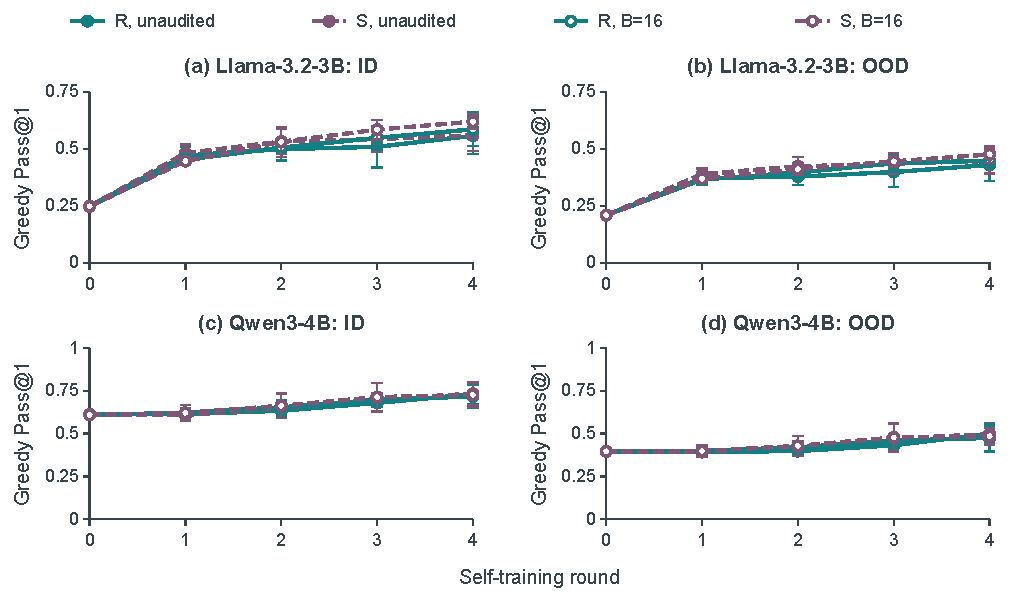
\includegraphics[width=0.82\textwidth]{figures/combined_graph_accuracy/graph_accuracy.pdf}
\caption{Four-round graph self-training for \textbf{Llama-3.2-3B (a--b)}
and \textbf{Qwen3-4B (c--d)}, with ID on the left and OOD on the right.
Both selection arms improve in mean. Llama's audited $R/S$ endpoints
reach $0.586/0.620$ ID and $0.449/0.476$ OOD, exceeding unaudited means;
Qwen's audited endpoints reach $0.718/0.727$ ID and $0.475/0.485$ OOD,
below unaudited means (Table~\ref{tab:audit-results}).
Auditing uses 16 correctness queries per arm-round.
Bars are pointwise 95\% block-$t$ intervals over five blocks on
2,000 ID and 1,000 OOD questions. Round-zero checkpoints are not
independent replications; each training round comprises multiple optimizer steps.
Qwen3-1.7B results appear in Appendix~\ref{app:qwen-four-round}.}
\label{fig:graph-four-round}
\label{fig:update}
\label{fig:qwen4b-four-round}
\end{figure*}


\paragraph{Evaluation and separate studies.}
The base and all 40 trained checkpoints per condition receive greedy
evaluation on the same 2,000 ID and 1,000 OOD questions.
For $N$ test questions, we define
$\mathrm{Pass@1}=N^{-1}\sum_{i=1}^{N}c(x_i,\hat y_i)$,
the fraction answered correctly, where $\hat y_i$ is the single greedily
decoded answer to $x_i$ and $c$ is the exact correctness indicator. Error is
$1-\mathrm{Pass@1}$; target rate is the fraction of all answers exhibiting
the target error. Descriptive 95\% block-$t$ intervals use five block means
or paired differences, conditional on these questions and without
multiplicity adjustment. Fixed-reference $h^T\Delta\theta$ is diagnostic,
not task risk. Separate one-step comparisons use the same three models,
five paired blocks, matched inputs, and dedicated reference gradients and
null baselines (Section~\ref{sec:lora}; Table~\ref{tab:one-step-heldout}).
Models are analyzed separately. Validation and computing resources are
described in Appendices~\ref{app:h100-results} and~\ref{app:cost}.
